\chapter{Solução proposta}\label{chap:solucao}

O trabalho em questão tem como objetivo a implementação do mecanismo que propaga os eventos de descoberta, conexão e desconexão que ocorrem no \stwopa do \mhub até a camada de aplicação do \cddl, de forma que os desenvolvedores possam projetar aplicações que se adaptem a tais eventos.
Visto que o \cddl somente exportava à camada de aplicação, eventos de leitura de dados de contexto.

Significando que dentre todos os objetos do tipo \sensordata criados no \stwopa, apenas aqueles com atributo ``\texttt{action}'' assumindo valor ``\texttt{READ}'' geravam eventos no \cddl que podiam ser percebidos pela aplicação (vide \autoref{subsub:s2pa}).

Este fato implica em algumas limitações no desenvolvimento de aplicações.
Imaginando um cenário onde uma aplicação necessite de certos dados providos por um \smartobj--- alocando recursos computacionais para processa-los.
Em uma eventual desconexão com o \smartobj, o fluxo de dados do sensor cessaria de ser entregue à aplicação, contudo, nenhum fluxo ou notificação do evento de desconexão em si seria entregue.
Tal aplicação não poderia decidir se o interrompimento do fluxo de dados se deu: devido a uma mudança na latência do envio de dados por parte do sensor, ou por uma desconexão; não podendo então decidir sobre a necessidade da desalocação de recursos.

Outra classe de aplicações de \iomt que seriam prejudicadas, são aquelas que interagem com \smartobjs no ambiente por outros meios além de conexões.
É o caso de aplicações de localização \textit{indoor} baseadas em \beacons \bluetooth, onde os \beacons são dispostos no interior de ambientes físicos e permanecem realizando \broadcast de sua presença.
Os dispositívos móveis não realizam tentativas de conexão, apenas percebem a presença destes \smartobjs e utilizam a intensidade do sinal capturado no momento.

Vale ressaltar que a implementação também deve permitir que tais eventos possam estar disponíveis para outras aplicações que estejam interessadas, utilizando para isso o \mqtt.
Ou seja---caso configurado desta forma---uma aplicação \mhubcddl pode mudar seu comportamento baseado em eventos que foram disparados a partir de interações entre \smartobjs e \smartphones remotos.

\section{Metodologia} \label{sec:metodologia}

O desenvolvimento do componente de \software foi realizado utilizando a metodologia ágil \textit{Feature-driven development}~\cite{coad:luca:lefebvre:1999}, dividido nas seguintes etapas:

\begin{alineas}
	\item transporte dos eventos gerados no \stwopa para o \cddl;

	\item definição de uma estrutura de tópicos onde os eventos serão publicados pelo \cddl, e posteriormente subscritos pelas aplicações interessadas;

	\item criação de uma \api para o consumo dos eventos.
\end{alineas}

Dentre as características que se considerou importantes, decidiu-se realizar a avaliação de desempenho e acurácia da solução.
As avaliações são realizadas através de simulações de cenários de uso, estes estão descritos no \autoref{chap:avaliacao}.

Como métricas da avaliação de desempenho, mede-se o tempo entre a ocorrência do evento e a sua respectiva notificação na camada de aplicação. Já as métricas de acurácia consistem na verificação da quantidade de notificação de eventos em relação a quantidade de eventos gerados.

\section{Requisitos de \software}

\subsection*{Requisitos funcionais}

Os requisitos funcionais definidos para a solução são:

\begin{alineas}
	\item notificação de eventos de descoberta, conexão e desconexão de \smartobjs para a camada de aplicação do \software;

	\item separação dos fluxos de eventos, provendo uma \api que permita a aplicação registrar interesse em cada tipo de evento individualmente;

	\item permitir que os eventos sejam acessíveis tanto para a aplicação que os gera, quanto para outras aplicações que registrem interesse;

	\item fornecer uma \api assíncrona para o recebimento de cada notificação dos eventos desejados.
\end{alineas}

\section{Implementação}

Esta seção descreve os detalhes de implementação da solução, abordando todos os tópicos descritos na \autoref{sec:metodologia}.

\subsection{Propagação de eventos do \stwopa para o \cddl}

Como descrito na \autoref{subsub:s2pa}, o \mhub encapsula todos os eventos em objetos do tipo \sensordata, estes objetos devem então ser propagados para o \cddl.
O \stwopa comunica-se com o \cddl através do componente \qocevaluator, como pode ser observado na \autoref{fig:mhub-cdll-architecture}~\cite{gomes:2017}.

A comunicação entre os componentes é feita através da biblioteca \eventbus\footnote{\url{http://greenrobot.org/eventbus/}}.
O \eventbus é uma biblioteca de eventos de código livre escrita em Java para a plataforma \android utilizando o padrão \pubsub, fornecendo um mecanismo central de comunicação simplificando a interação entre componentes da aplicação.

O \stwopa foi modificado então para publicar cada \sensordata no \eventbus, enquanto o \qocevaluator registra interesse em receber objetos do tipo \sensordata publicados no \eventbus.
O que efetivamente transfere todos os eventos gerados pelo \stwopa ao \cddl.

\subsection{Separação dos fluxos de eventos}

Como todos os dados publicados pelo \cddl são do tipo \msg, decidiu-se manter este padrão, de forma a manter a retrocompatibilidade e assim continuar suportando as aplicações antigas.
Ao invés de utilizar a estratégia adotada pelo \mhub (utilizar um atributo que identifica que tipo de evento o objeto está representando), adotou-se uma estratégia baseada em orientação a objetos.
Foram criadas três novas classes que herdam os atributos de \msg, são elas:

\begin{alineas}
	\item \objfoundmsg: Para os eventos de descoberta;
	\item \objconnectedmsg: Para os eventos de conexão;
	\item \objdisconnectedmsg: Para os eventos de desconexão.
\end{alineas}

Com esta abordagem é possível utilizar a \api e métodos existentes, valendo-se do mecanísmo de polimorfismo da orientação a objetos.
Ao receber um \sensordata, o \qocevaluator faz o seguinte: identifica, utilizando o atributo \texttt{action}, que tipo de evento ele representa; instancia um objeto de um dos tipos descritos anteriormente; e o publica no \broker \mqtt como um objeto do tipo \msg.

Aplicações que estão interessadas em certo tipo de serviço receberão uma instância de \msg a cada evento gerado.
Como ela é superclasse das anteriores, a aplicação pode verificar em tempo de execução se determinado objeto é instância das classes mais especializadas, como é mostrado no \autoref{lst:polymorphism}.

\lstinputlisting[float=htb, label=lst:polymorphism, caption=Uso das classes mais especializadas em conjunto com a \api existente]{code/Polymorphism.java}

\subsection{Definição da estrutura de tópicos}

De forma a gerar fluxos diferentes para cada evento, e permitir consultas mais expressivas, o \qocevaluator deve publicar cada mensagem gerada em um tópico específico, de acordo com o tipo de evento que este representa.

A estrutura de tópicos propósta para publicação de eventos de descoberta, conexão e desconexão segue o seguinte padrão:
\[
	\underbrace{\bm{\mathsf{domain}}\vphantom{p}}_{\text{\textsf{identificador do \cddl}}}
	\bm{/}
	\underbrace{\bm{\mathsf{clientId}}\vphantom{p}}_{\text{\textsf{identificador do cliente}}}
	\bm{/}
	\underbrace{\bm{\mathsf{eventTopic}}}_{\text{\textsf{identificador do tipo de evento}}}
\]
Onde:

\begin{alineas}
	\item \emph{domain}: É um prefixo que identifica todas as mensagens publicadas pelo \cddl, isto permite que seja possível identificar as mensagens pertencentes ao \middleware, mesmo que um \broker público seja utilizado;
	\item \emph{clientId}: É um identificador da aplicação cliente que gerou tal mensagem. Este valor é informado pelo desenvolvedor ao iniciar o \cddl;
	\item \emph{eventTopic}: Identificador único para cada tipo de evento, ou seja, para os evento de descoberta, conexão e desconexão.
	\begin{alineas}
		\item \texttt{object\_found\_topic}: Para os eventos de descoberta;
		\item \texttt{object\_connected\_topic}: Para os eventos de conexão;
		\item \texttt{object\_disconnected\_topic}: Para os eventos de desconexão.
	\end{alineas}
\end{alineas}

Foram então adicionados métodos à interface \texttt{Subscriber} que permitem que a aplicação registre interesse em cada tipo de evento gerado através de interações entre \smartobjs o próprio dispositivo móvel em que executa, e também métodos que permitem que a aplicação receba eventos gerados por outras aplicações. Estes métodos inscrevem a aplicação no tópico \mqtt específico.

A fim de se inscrever em eventos gerados por outras aplicações \mhubcddl, faz-se uso dos caracteres coringa do \mqtt descritos na \autoref{subsec:mqtt-topics}. Fazendo com que a aplicação se inscreva em tópicos com o seguinte padrão: \texttt{domain/+/eventTopic}.

Caso a aplicação não possua o requisito de compartilhar os eventos gerados por ela com outras aplicações, pode-se utilizar o \ubroker embarcado disponível na plataforma \mhubcddl.

\begin{figure}[htb]
	\centering
	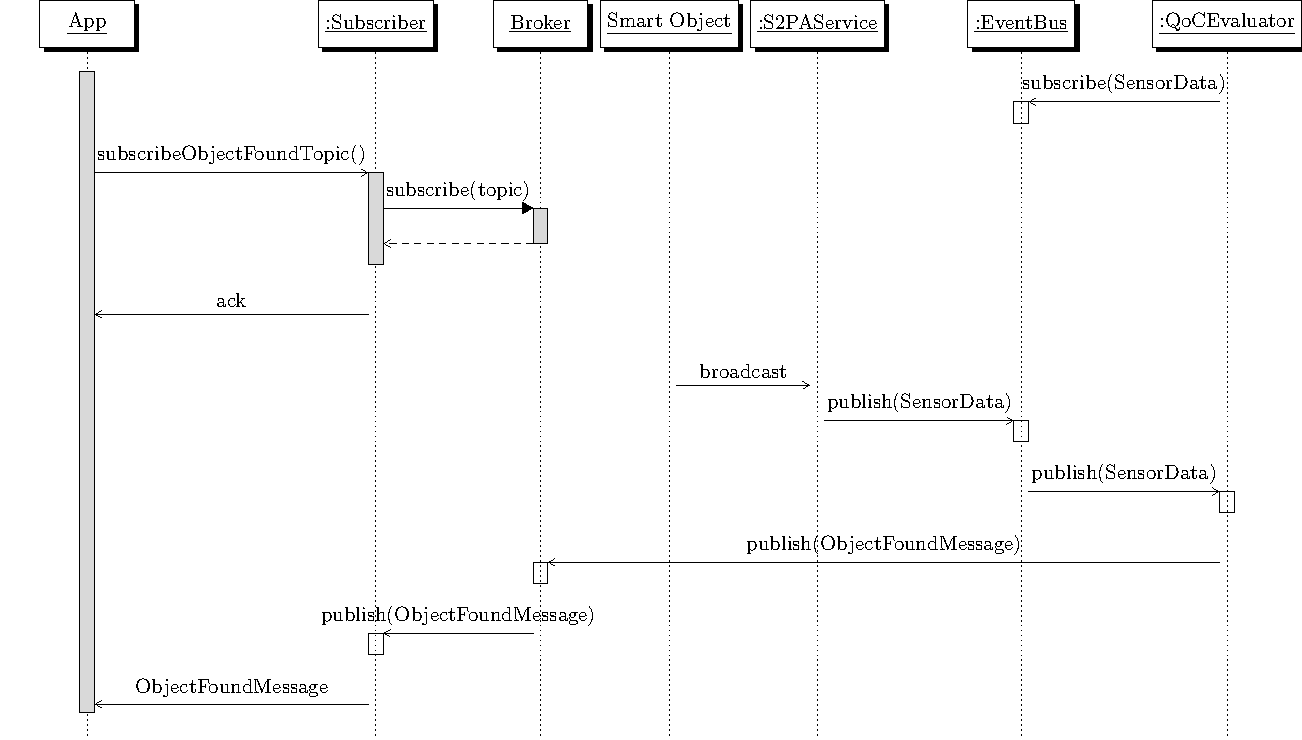
\includegraphics[width=0.95\textwidth]{img/solution-sequence.pdf}
\end{figure}

